\documentclass[12pt]{article}

\usepackage{tikz}
\usepackage{geometry}

\usetikzlibrary{mindmap}

\pagestyle{empty}

\geometry{landscape, margin=1cm}


\begin{document}
\begin{center}
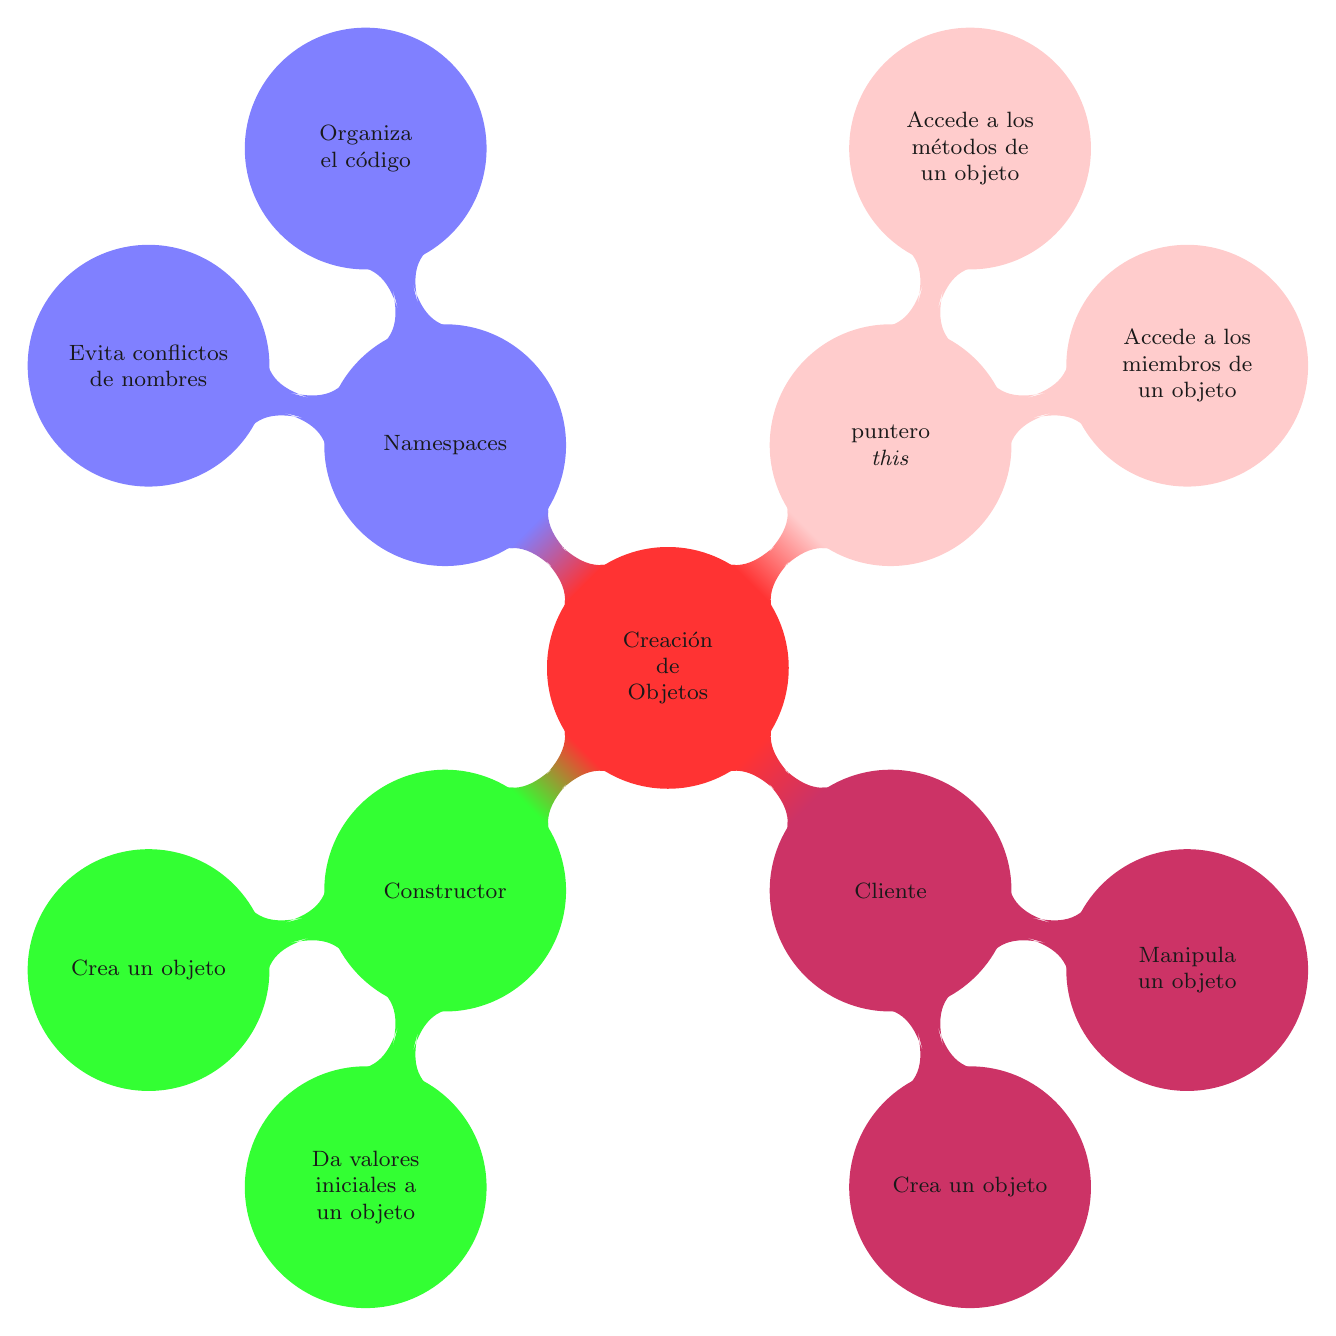
\begin{tikzpicture}[small mindmap, grow cyclic, every node/.style=concept, concept color=red!80, text=black!90, minimum size=3.0cm,
    level 1/.style={level distance=4.5cm,sibling angle=360/4},
    level 1/.style={level distance=4.0cm,sibling angle=360/4},
    level 2/.style={level distance=3.9cm,sibling angle=60},
    level 3/.style={level distance=3.5cm,sibling angle=60},
    ]

    \node{Creación\\de\\Objetos}
    child [concept color=green!80] { node {Constructor}
        child { node {Crea un objeto} }
        child { node {Da valores iniciales a un objeto} }
    }
    child [concept color=purple!80] { node {Cliente}
        child { node {Crea un objeto} }
        child { node {Manipula un objeto} }
    }
    child [concept color=pink!80] { node {puntero\\\textit{this}}
        child { node {Accede a los miembros de un objeto} }
        child { node {Accede a los métodos de un objeto} }
    }
    child [concept color=blue!50] { node {Namespaces}
        child { node {Organiza el código} }
        child { node {Evita conflictos de nombres} }
    }
    ;
\end{tikzpicture}
\end{center}
\end{document}
